\documentclass{article}
\usepackage{amsmath}
\usepackage{hyperref}
\usepackage{graphicx}
\usepackage{adjustbox}
\usepackage{caption}
\usepackage{subfigure}
\newcommand{\tabincell}[2]{\begin{tabular}{@{}#1@{}}#2\end{tabular}}
\begin{document} %This is where document begins
\begin{titlepage}
\title{EE 232E \\Graphs and Network Flows\\Project 1\\Winter 2016} 
\author{Liqiang Yu, Rongjing Bai, Yunwen Zhu\\
904592975, 204587519, 104593417}  %change your ID here
\date{05-14-2016}
\end{titlepage}
\maketitle
\newpage
\tableofcontents
\newpage

\section{Problem 4}
After deleting the core node 1, the personal network of core node 1 is shown in figure \ref{fig:p4_1}
\begin{figure}[htbp]
\centering
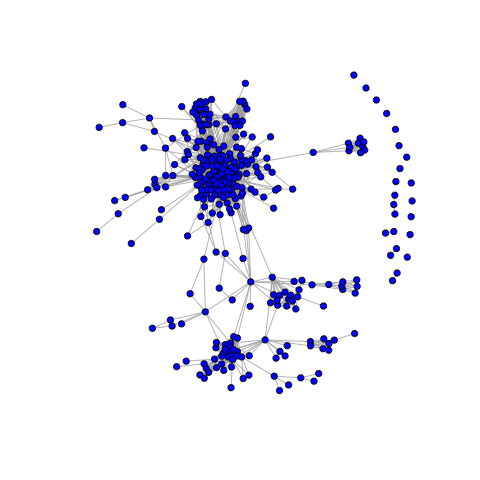
\includegraphics[width=.8\textwidth]{p4_1.png}
\caption{in degree distribution}
\label{fig:p4_1}
\end{figure}
After applying Fast Greedy, Edge Betweenness and Infomap algorithms to the personal network of core node 1 after the deletion, we can explore the community structures and compare them with the network before the deletion. The results are shown in figure \ref{fig:p4_2}. The left column are the community structures after applying three kinds of algorithms and the right column are the comparison results of the community distribution before and after the deletion.\\
\\
 From figure \ref{fig:p4_2} we can see that edge betweenness and infomap method almost produced the same results, but fast greedy produced the distribution that moved right a little bit. \\
 \\
 Moreover, the modularity results before and after the deletion are shown in table \ref{tb:p4}. From the results we can see that infomap produced exactly the same results, however fast greedy and edge betweenness both produced larger results after the deletion, which makes sense. Because the modularity is, quoted from wikipedia, "designed to measure the strength of division of a network into modules (also called groups, clusters or communities). Networks with high modularity have dense connections between the nodes within modules but sparse connections between nodes in different modules." After deleting the core node, which is pivot node of the its personal network, the network should be easier to divide into modules and therefore the modularity should increase.
\begin{figure}[htbp]
\centering
%\captionsetup{justification=centering,margin=2cm}

\subfigure{
\begin{minipage}[b]{0.4\textwidth}
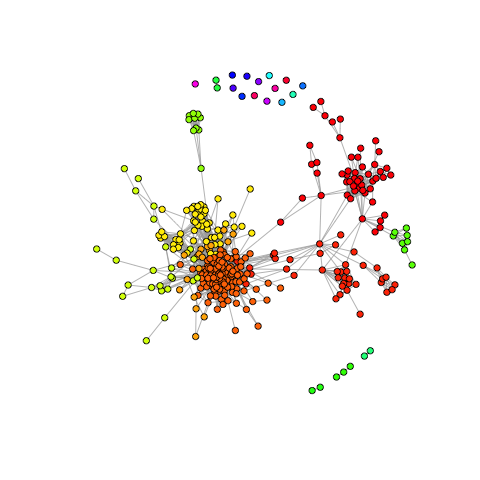
\includegraphics[width=1\textwidth]{p4_2_fgc.png} \\
\caption*{The community structure for fast-greedy method}
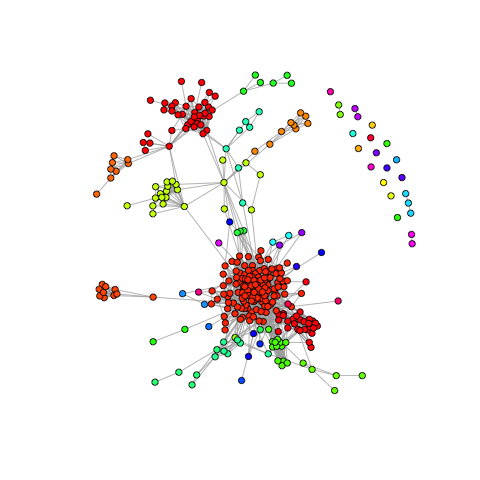
\includegraphics[width=1\textwidth]{p4_2_ebc.png}\\
\caption*{The community structure for edge-betweenness method}
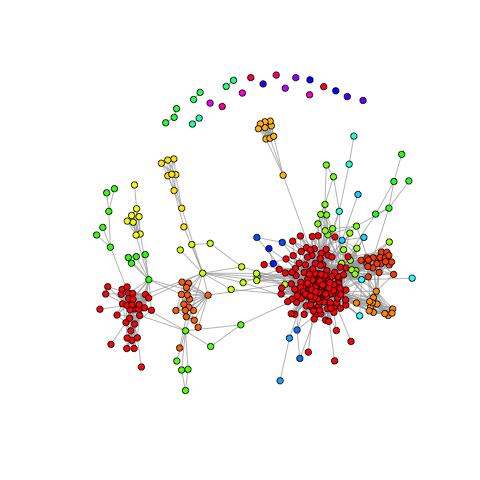
\includegraphics[width=1\textwidth]{p4_2_ifc.png}
\caption*{The community structure for infomap method}
\end{minipage}
}
\subfigure{
\begin{minipage}[b]{0.4\textwidth}
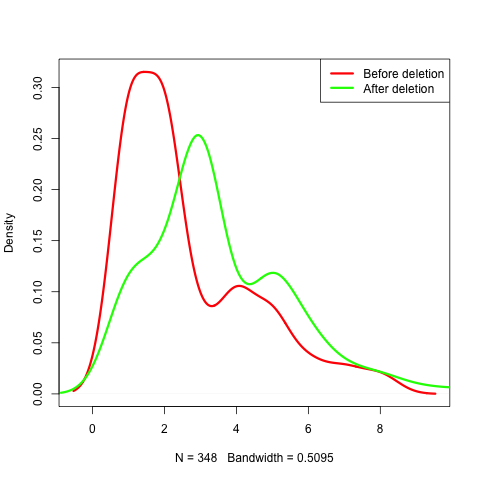
\includegraphics[width=1\textwidth]{density_compare_fgc.png} \\
\caption*{The comparison results for fast-greedy method}
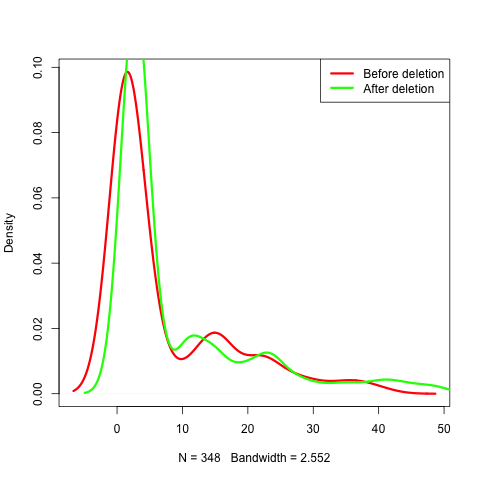
\includegraphics[width=1\textwidth]{density_compare_ebc.png}\\
\caption*{The comparison results for edge-betweenness method}
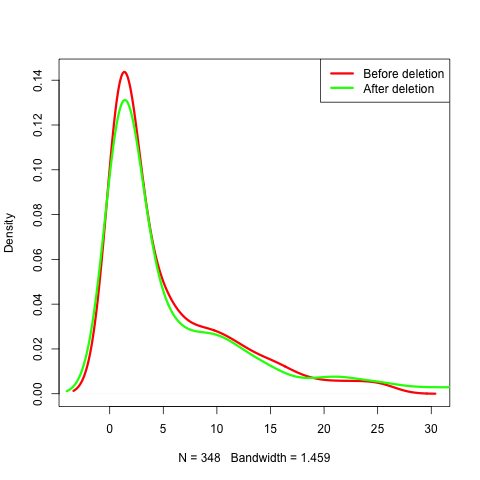
\includegraphics[width=1\textwidth]{density_compare_ifc.png}
\caption*{The comparison results for infomap method}
\end{minipage}
}
\caption{}
\label{fig:p4_2}
\end{figure}

\begin {table}[htbp]
\caption{The modularity comparison results}
\begin{adjustbox}{center}
\label{tb:p4}
\begin{tabular}{|c|c|c|c|}
\hline
&fast-greedy &edge-betweenness &infomap\\
\hline
Before deletion&0.4131014&0.3533022&0.4180077\\
\hline
After deletion&0.4418533& 0.4161461& 0.4180077\\
\hline
\end{tabular}
\end{adjustbox}
\end{table}

\section{Problem 6}
In this problem, we choose to use the cluster coefficient and density to define two types of communities in the 41 personal networks. We try to find the community indices that have maximal and minimal results and compare them to draw the conclusion.
\subsection{Cluster Coefficient}
\subsubsection{Local Cluster Coefficient}
The local clustering coefficient of a vertex in a graph quantifies how close its neighbors are to being a clique. A graph $G=(V,E)$ formally consists of a set of vertices $V$ and a set of edges $E$ between them. A edge $$
\subsection{Density} 
\end{document}
